% --------------------------------------------------------------------

\chapter[Eruptive and Explosive Transients]{Explosive Transients}
\def\chpname{transients}\label{chp:\chpname}

% \noindent {\it
% Mike Lund, Ashish Mahabal, Stephen Ridgway, Lucianne Walkowicz, Rahul Biswas, Michelle Lochner, Jeonghee Rho, Eric Bellm, Federica B. Bianco...
% }

Chapter editors:
\credit{ebellm},
\credit{fedhere},

Contributing Authors:
\credit{AshishMahabal},
\credit{StephenRidgway},
\credit{ohadshemmer},
\credit{fedhere},
\credit{paulaszkody},
\credit{nathansmith},
\credit{tommatheson}

% --------------------------------------------------------------------

\section{Introduction}


Explosive and eruptive transients include a diverse ensemble of
object, diverse both physically and phenomenolocigally. Transients
such as novae, supernovae (SNe), and gamma-ray bursts (GRBs) probe the
final stages of stellar evolution, Tidal Disruption Events (TDEs),
Gamma Ray Bursts (GRBs), Cataclysmic Variables (CVs) give us the
opportunity to study compact and binary objects, massive star
eruptions allow us to understand mass loss mechanisms, and chemical
enrichment. Transients impact the evolutionary history of the
Universe. The brightest transients (GRBs, TDEs, SNe) are light beams
that can be seen over cosmic distances, and some transients (Type Ia
SNe in the first place) are cosmological tracers.  Cadence choices
will determine LSST's ability to discover, classify, and characterize
these events. However, different types and time scales of phenomena
will benefit from different sampling strategies---sometimes
significantly different, and at times orthogonal.  Competing
objectives described in this chapter are at the heart of LSST
observing strategy and cadence design.

When evaluating a particular observation or series of observations in
light of how they perform for a specific science case, it may be
helpful to think of metrics as lying along a continuum between
discovery and characterization. Discovery requires a minimum amount of
information to recognize an event or object as a candidate of
interest, which necessarily involves some level of bare-bones
characterization; rich characterization, on the other hand, implies
that an event may not only be recognized as a candidate of interest,
but basic properties of the event or object may be determined from the
LSST observations (including but not limited to the classification of
the event). The level of characterization accessible through LSST data
will of course evolve with time for all the transients that have
characteristic time scales longer than a few days.

Transient events may benefit from substantial temporal sampling
(matched to the time constant of the event) with color information
(perhaps contemporaneous) to support characterization and
classification, obtained over the limited duration of interest.
Transient events slower than $\sim$ weeks may be adequately sampled by
a uniform LSST cadence.  Faster events may require special scheduling
strategies.  For some event types, LSST can only be expected to
provide a discovery service, and followup will necessarily be
performed elsewhere.  For some events, for example detecting LIGO
counterparts, a serendipitous discovery is extremely unlikely, but
enabling a TOO program would provide the opportunity for LSST to
contribution significantly to this science.

%The interpretation of a given metric along this continuum has
%implications for the subsequent action and analysis required,
%particularly as regards possible follow-up observations with other
%facilities.

We consider a non-exhaustive set of ``astronomical transients'' in the
paragraphs that follow.

\subsection{Targets and Measurements}
\label{sec:\chpname:targets}

%The class of transients includes a heterogeneous assortment of objects
%and phenomena.
The table below is a \emph{non-exhaustive} list of
phenomena we are referring to as \emph{Eruptive and Explosive
  transients} in this document.

\begin{center}
\begin{tabular}{| p{3cm} | p{8cm} | l | l |}
    \hline

    Transient Type & Science drivers & Amplitude & Time Scale\\
\hline

Flare stars & Flare frequency, energy, stellar age & large & min \\

X-ray Novae & Interacting binaries, stellar evolution, SN progenitors, nuclear physics & large & weeks \\

Cataclysmic variables & Interacting binaries, stellar evolution, compact objects & large & min - days\\

LBV variability & Late stages stellar evolution, Mass loss, SN progenitors & large & weeks-years\\

Massive star eruptions & Late stages stellar evolution, Mass loss, SN progenitors & extreme & weeks-years\\

SN & stellar evolution, feedback, chemical enrichment, cosmology & large & days - months \\

GRBs & SN connection, stellar evolution, cosmology & large & min - days\\

TDEs & Massive BH demographic & large & days\\

LIGO detections & EM characterization & unknown & unknown\\

Unknown & Discovery & unknown & unknown\\

 \hline \end{tabular}
 \end{center}


{\bf What else?}


%templates and stacks

%confusion 

%


% --------------------------------------------------------------------


\subsection{Transient time scales}

For very short lived phenomena (stellar flares, CV outbursts, GRBs,
LIGO events) the main function of LSST will be to provide discoveries
and/or simple characterization.  Followup to discovery/identification,
if required, will surely take place elsewhere.

LBV's, Gap transients??

SN fall in an intermediate time range.  LSST will provide
multiple visits in multiple filters during the typical SN duration
(months).  This sampling may be insufficient for many science
objectives.  However, moderate, and feasible, changes to LSST
observing strategy, may enhance the sampling for part of the sky part
of the time, greatly improving the usefulness of SN observations. 
Metrics that assess the discovery rate of SN are included in the
cosmology chapter. Here we are interested in assessing the ability of
LSST to discriminate SN from other transients, SN subtypes from one
another, and to identify particularly interesting SNe: for example
those that show signature of shock break-out, or companion interaction
in the early light curve, and would be candidates for \emph{flash
  spectroscopy} follow-up (ref here). In addition metrics that
quantify LSST's ability to constraint SN physics in a statistically
large sample of SN are needed (offered hopefully).


TDEs, whose fading time-scale is much more gradual
(over weeks to months) than the rise time-scale and we want to asses -
through a metric - how many are detected while still on the
rise. Ref. Science Book: 10.6.1. Also ref. recent papers.

A phenomenon that falls under this document's definition of explosive
transients, but is not discussed here, is AGN. AGN are likely to be
sampled with sufficient resolution by a uniform LSST cadence and they
are discussed in Chapter \ref{chap:AGN}.

In addition we hope that LSST will provide a wealth of serendipitous
discoveries of yet-to-be-observed transients.  An ideal transient
discovery survey would include heavy coverage of all time scales. LSST
will cover longer time periods well, but will have to make some
choices of emphasis in coverage of shorter time-scales. (metric
here??)


In the paragraphs that follow we will use case studies to asses:

\begin{itemize}
\item
The discerning power of a given LSST observing cadence. For this topic
we will address the ability to distinguish LBVs, SNe, and TDEs.
\item
The ability to identify an object of interest for follow-up and
trigger prompt follow-up observations. For this topic GRBs are used as
a case study.
\item
The insight that a cadence gives into a single transient class. The
case study will be massive star eruptions.
\item 
The statistical constraints to a transient class that can be obtained
over the course of the LSST survey, from the LSST survey data alone
(assuming a successful classification). SN Ia early interaction
signatures or IIb shock break-out.
\end{itemize}

In this chapter we focus on LSST's potential to advance the science of
eruptive and explosive transients; the use of SNe for cosmology is
discussed in \autoref{chp:cosmo}.


% --------------------------------------------------------------------

\subsection{Metrics}
\label{sec:\chpname:metrics}

\begin{center}
\begin{tabular}{| p{5cm} |p{10cm} |}
\hline Metric & Description\\ \hline SNe & Number of events adequately
sampled\\ Serendipity & Histogram of median visit series length vs
maximum visit spacing within the series\\ \hline \end{tabular}
 \end{center}


%%WHO WROTE THIS? I AM NOT SURE WHAT THIS METRIC DESCRIPTION MEANS
The metrics for SNe will be highly specialized and based on the best
available understanding of SN light curve analysis and the expected
event population.

The suggested metric set for serendipity is based on the simple-minded
idea that a novel transient will be characterized by a band-limited,
finite waveform, and that a useful observation series will consist of
a series of samples extending over the duration of the event, with at
least critical sampling of the fastest variations.  Since for some
event durations the number of useful time series will be small, it may
be useful to look not at the median length, but the median length of a
subset size preselected as possibly useful (e.g. the$10^3$ longest
series).

Lund et al. (2015; \url{http://arxiv.org/pdf/1508.03175.pdf}) discuss
three metrics that have been incorporated into the MAF. Two of these
metrics deal explicitly with time variable behavior: a) observational
triplets, and b) detection of periodic variability. While in this
chapter w do not deal with periodic phenomena, the first of these
metrics is useful to generically assess the performance of LSST for
transients of all types. More specialized transients metrics can be
obtained by simply using a more realistic light curve shape. A metric
that uses input ASCII files is provided, to enable the assessment of
discovery and characterization of an arbitrarily shaped transient.

\subsubsection{Observational triplets (TripletMetric)}

This metric provides a means of evaluating whether a transient event
on some time scale of interest has been detected, by testing for a
sequence of three observations. The object must be detected in
quiescence, followed by two subsequent detections above some
threshold; this sequence of observations allows the magnitude of the
change to be measured, as well as its time scale.

This metric may be used for a variety of astrophysical phenomena, in
particular transient events on variable objects (e.g. novae, stellar
flares), in that it is general with respect to the amplitude of the
brightness variation as well as the time scale of said change. The
requirement of a detection prior to outburst does constrain it to
objects that have already been detected in quiescence (in other words,
not necessarily ``true'' transients), although there may be some cases
where this is not the case (e.g. a supernova occurring on a previously
detected galaxy). In practice, the time lapse between the first and
second and second and third observations must be comparable (between
10$^2$ and 10$^5$ seconds) for discovery. This metric may be
calculated for a given OpSim run and then further reduced to a
histogram in logarithmic time bins; the minimum number of bins to
construct an interesting sample of objects is source-dependent.

\subsubsection{Transient Metric (transientAsciiMetric)}

Calculate what fraction of transients would be detected using an ASCII
input file for the light curve.

\subsection{Proposed Metrics}

The following is a raw list of metric ideas; these need specificity
and further description.

The triplet metric may also be altered to include filter constraints,
such that the triplets are drawn from a single filter or subset of
filters.

Color evolution constraint: triplets of observations in a specific
color (really requirement of two triplets in multiple filters)

  2D Histogram of delta t?s between observations constituting a triplet

Histogram of median visit series length vs maximum visit spacing
within the series

Number of events adequately sampled

% --------------------------------------------------------------------

\subsection{OpSim Analysis}
\label{sec:\chpname:analysis}

Analysis shows that current simulations provide  poor coverage in any one filter for transient events longer than a deep drilling session ($\sim$30 minutes) and shorter than $\sim$ weeks.

Simulated performance for SN observations must be analyzed for both
main survey and mini-survey (deep drilling) productivity.  It is
considered that current simulated schedules give inadequate
performance for SN science.



% --------------------------------------------------------------------

\subsection{Discussion}
\label{sec:\chpname:discussion}

Community studies are providing improving SNe metrics, and continuing
communication between the SN and LSST communities is essential to
tuning the observing strategy to deliver the SN time series that are
needed and possible.

Improving LSST science return for SNe will also improve sampling of
all transients with similar or somewhat shorter characteristic times.
Non-uniform survey strategies (rolling cadence) can significantly
improve the LSST performance for faster transients.  Interpretation of
multiple filters for novel events may be powerful, or problematic,
since color may be uncertain.

Some insight into fast transients may be available from image pairs or
triples (as opposed to more complete series).  These include the pair
of images in a visit - which could be useful in studying the rise time
of an extremely fast event.  This includes the characteristic grouping
of visits (typically 0.5 to 1.0 hour separation) planned for purposes
of identifying asteroids.  It also includes fortuitous multiple
sampling due to field overlap, providing additional sampling, which
may be random or systematic, depending on the scheduling, on a time
scale of minutes to hours.  The sampling benefits of this fortuitous
overlap have not yet been investigated.


\navigationbar

% --------------------------------------------------------------------

% ====================================================================
%+
% SECTION:
%    sn.tex  
%
% CHAPTER:
%    transients.tex  
%
% ELEVATOR PITCH:
%    Explain in a few sentences what the relevant discovery or
%    measurement is going to be discussed, and what will be important
%    about it. This is for the browsing reader to get a quick feel
%    for what this section is about.
%
% COMMENTS:
%
%
% BUGS:
%
%
% AUTHORS:
%   Federica Bianco (@fedhere)
%
% ====================================================================

\section{Cataclismic Variables}
\def\secname{CVtransients}\label{sec:\secname} % For example, replace "keyword" with "lenstimedelays"

\credit{paulaszkody}, \credit{fedhere} % (Writing team)

Cataclysmic Variables (CVs) encompass a broad group of objects
including novae, dwarf novae, novalikes, and AM CVn systems, all with different
amplitudes and rate of variability. The one thing they all have in
common is active mass transfer from a late type companion to a
white dwarf. The variability ranges from minutes (due to the flickering in
dwarf novae and novalikes, the pulsations in accreting white dwarfs in
the instability strip, or the orbital periods of AM CVn systems), to
hours (for the orbital periods of novae, dwarf novae and novalikes) to
days (for the normal outburst lengths of dwarf novae) to 
weeks (for the outburst length of superoutbursts in short orbital period
dwarf novae and the outburst recurrence time of normal outbursts in short
orbital period dwarf novae) to months (for the outburst recurrence time of 
longer period dwarf novae, various state changes in novalikes and the decline 
in novae) and, finally, to years (for the outburst recurrence timescales of the 
shortest period dwarf novae and the recurrence times in recurrent novae). The 
amplitudes range from tenths of mags for flickering and pulsations to 4 mags 
for normal dwarf novae and changes in novalike states up to 9-15 mags for the 
largest amplitude dwarf novae and regular novae.

These large differences make correct classification with LSST difficult
but necessary in order to reach goals of assessing the correct number
of types of objects for population studies of the end points of
binary evolution. Multiple filters (especially the blue $u$ and $g$) 
along with amplitude and recurrence of variation provide the best
discrimination, as all CVs are bluer during outburst and high states of
accretion. Long term evenly sampled observations can provide indications
of the low amplitude random variability and catch some of the more frequent
outbursts but higher sampling is needed to determine whether an object
has a normal or superoutburst, to catch a rise to outburst or to a
different accretion state or to follow a nova. Novae typically
have rise times of a few days while the decline time and shape provide
information as to the mass, distance and composition. The time to decline
by 2-3 magnitudes is correlated with composition,

***FED: what is a range of time scales for this decline? days? months?

WD mass and location in
the galaxy, thus enabling a study of Galactic chemical evolution.  As with SN, 
the diagnostic power for all these systems rests on color and sampling.   

The metrics rely on a given cadence to provide shape and recurrence time
of large variations that will distinguish between new novae, dwarf novae
outbursts and identify hig vs low states, as well as available blue colors to 
distinguish low amplitude variability that would indicate new pulsators or 
novalikes. The population studies rely on the numbers of long orbital period 
(low amplitude, wide outbursts) vs short orbital period (patterns of short 
outbursts followed by larger, longer superoutbursts) dwarf novae at different 
places in the galaxy, as well as the numbers of recurrent (1-10 yrs) vs normal 
novae (10,000 yrs, about 35/galaxy/yr). Objects particulary worthy of 
discrimination for later followup are the numbers of CVs containing highly 
magnetic white dwarfs. These can be identified by a metric of 10 yrs of data on
a large sample where the magnitude for a majority of the years is a faint (low)
state and a small percentage of time is a bright (high) state, combined with a 
red color (due to cyclotron emission from the magnetic accretion column).


% --------------------------------------------------------------------

% ====================================================================
%+
% SECTION:
%    sn.tex  
%
% CHAPTER:
%    transients.tex  
%
% ELEVATOR PITCH:
%    Explain in a few sentences what the relevant discovery or
%    measurement is going to be discussed, and what will be important
%    about it. This is for the browsing reader to get a quick feel
%    for what this section is about.
%
% COMMENTS:
%
%
% BUGS:
%
%
% AUTHORS:
%   Federica Bianco (@fedhere)
%
% ====================================================================

\section{Supernovae as transients}
\def\secname{SNtransients}\label{sec:\secname} % For example, replace "keyword" with "lenstimedelays"

\credit{fedhere} % (Writing team)

Supernovae (SNe) are the final dramatic stages of stellar life. SNe include a diverse set of phenomena: explosion of low mass stars in binary systems, thermonuclear SN or SN Ia (also discussed in \ref{sec:supernovae}), and explosion of high mass stars, Core collapse (CC) SNe. Phenomenologically the observable of the explosion are themselves diverse.  The transient duration ranges between weeks and months, possibly years. The electromagnetic energy radiated ranges between $\sim0.1$ (faintest CC SNe), to $\sim1$ (SN Ia) and $\sim100$ (Superluminous SNe, SLSNe) ($\times 10^{49}$ erg), corresponding to absolute magnitudes at peak ranging between $\sim-19$ and $\sim-22$.

LSST's contribution to SNe studies can can be substantial, on many different aspects. The first crucial input will be discovery: we expect as many as $\sim 1000$ SN discoveries per night. The first step is then \emph{discrimination}, and the first question we need to answer, with a metric, is: will LSST photometry allow to distinguish the different types of SN to appropriately direct follow-up efforts?

When a large statistical sample of SNe is generated, LSST's photometry may allow to set constraints on the diversity of the sample, and thus inference on the diversity within the population of SN, which in turn may constrain the genesis of the explosion. Outstanding questions that can be answered statistically are: what is the percentage of SN Ia that arise from a \emph{single degenerate} progenitor system (a CO WD-WD binary), from a {\emph single degenerate} system (a WD-MS or WD-RG binary), or a {\emph merger} (a WD-WD binary with a He and a CO WD) (citation). Answering this question may reduce the scatter in the Hubble diagram, if SNe from different progenitors are shown to require different standardization (citation). On the CC SN side: the diversity of SN subclasses, and the relationship between them (is there a phenomenological continuum or actually distinct classes, e.g. between IIp-IIL, IIb-Ib?) is yet to be understood. Individual well studied objects may answer these questions, for example individual SN Ia with tight constraints on the progenitor system show that both single and double degenerate progenitors exist (e.g. SN 2011fe, \citealt{Li2011}, and PTF 11kx, \citealt{Dilday11}). However, a statistical sample is suitable to set constraints on populations. Thus the question  we need to answer, with a metric, is: how much detail can be sacrificed in favor of sample size without compromising diagnostic power? And the diagnostic power relies on color and sampling: thus what is the trade-off between cadence in the same filter, and observations in different filters. Specifically, transients can be distinguished early from two photometric characteristics: rise time and color. There is a tension between these observables: obtaining colors relies of course on obtaining photometry in different bands at within short time scales, ideally simultaneously, although within a night is probably sufficiently close. However, assessing the rise slope is best done with a single filter, so prompt characterization also needs multiple epochs within a night, although separated by at least a few hours, in the same filter. That is: observing with differnt filters it is impossible (or very hard) to separate shape from color. Colors of course allow to learn a lot more about the statistical sample: as long as the epoch of peak is reliably assessed coadded lightcurves can be studeid (Bianco 2011).


Thus we envision 2 SN related metrics: 
\begin{itemize}
\item a metric that assess the ability of a cadence to distinguish between SNe among all transients, the ability to distinguish among SN subtypes, and within a subtype the ability to gauge how typical, or atypical (and thus worthy or particular attention) a SN is. 
\item a metric that works on a large sample (3-, 6-, 9-years of LSST data) and assess the ability to characterize the contribution of SN with specific features to the population: as a test case we will use the presence of an early blue excess for type Ia, signature of interaction with a companion, and the presence of an early blue escess signature of shock breakout for CC SNe.
\end{itemize}


% --------------------------------------------------------------------

% ====================================================================
%+
% SECTION:
%    grb.tex  % eg lenstimedelays.tex
%
% CHAPTER:
%    transients.tex  % eg cosmology.tex
%
% ELEVATOR PITCH:
%    Explain in a few sentences what the relevant discovery or
%    measurement is going to be discussed, and what will be important
%    about it. This is for the browsing reader to get a quick feel
%    for what this section is about.
%
% COMMENTS:
%
%
% BUGS:
%
%
% AUTHORS:
%    Phil Marshall (@drphilmarshall)  - put your name and GitHub username here!
%-
% ====================================================================

\section{Gamma-Ray Burst Afterglows}
\def\secname{grbs}\label{sec:\secname} % For example, replace "keyword" with "lenstimedelays"

\credit{ebellm} % (Writing team)

Gamma-ray bursts (GRBs) are relativistic explosions typically classified by the temporal duration of their initial gamma-ray emission: Long GRBs, that mark the endpoint of the lives of some massive stars, and short GRBs, believed to originate from the merger of binary neutron stars.
GRB emission is known to be beamed: the initial prompt gamma-ray emission is seen only for observers looking at the jet axis. The longer-wavelength X-ray, optical, and radio afterglow may be seen both by on- and off-axis observers.  The latter case is known as an orphan afterglow, due to the absence of gamma-ray emission.  
On- and off-axis afterglows are predicted to have different temporal signatures in the optical: On-axis events decay as a power-law until a jet break, while off-axis events should be fainter and show an initial rise 
Despite systematic searches, no convincing orphan afterglow candidates have yet been discovered, limiting our knowledge of the beaming fraction of GRBs and hence their true rates.
Well-sampled orphan afterglow lightcurves would also permit study of the GRB 
jet structure.

Because of their rarity, in all but one case \citep{2015ApJ...803L..24C} to date GRBs have been discovered using their prompt emission by hard X-ray or gamma-ray all-sky monitors.  
This selection imposes biases on the population of relativistic explosions we observe.  
Baryon-loading in the GRB jet---a ``dirty fireball'' \citep{2003ApJ...591.1097R}---can lead to on-axis events without gamma-ray emission.  Only one plausible candidate has been identified to date \citep{2013ApJ...769..130C}.  
Discovery of new dirty fireballs---if distinguished from off-axis events--would clarify the rates of these events and enhance our understanding of the diversity of stellar death.

LSST is the survey most capable of resolving these decades-old questions.  Due to its large aperture and etendue, LSST can detect faint, fast-fading, and rare cosmological events, potentially enabling population studies of the high-redshift universe.  
\citet{2015A&A...578A..71G} estimated LSST could detect 50 orphan afterglows each year, more than any other planned survey.

%deep survey helps due to time dilation

%beaming fraction and true rates; jet structure; dirty fireballs?
%GRB-SN connection; probe high-z star formation?

%other fast transients: Fast transients and SN shock breakout?  flash spectroscopy

% --------------------------------------------------------------------

\subsection{Target measurements and discoveries}
\label{sec:\secname:targets}

GRB afterglow discovery is among the science cases that places the greatest stress on the LSST cadence.  Because afterglows fade rapidly---dropping several magnitudes in the first few hours---high cadence observations are required to detect the fast fading.  
If an afterglow candidate can be recognized in real time, it will be possible to trigger TOO spectroscopy (to measure a redshift and confirm the event is cosmological), X-ray observations (to detect a high-energy counterpart), and additional photometry (to characterize the lightcurve evolution).  If there is no source at the location of the transient in the coadded reference image, two consecutive observations in the same filter separated by an hour or two are the minimum required to potentially trigger followup of a fast-fading event.  
However, a third or fourth observation in a single night---ideally in the same filter---would improve the purity of the sample.  Observations in other bands at high cadence are less useful because they require assumptions about the event's SED and its evolution to determine if a source is truly fading.

Distinguishing orphan afterglows from on-axis events (whether conventional GRBs or dirty fireballs) will also require more than two detections.  Orphan events may prove harder to recognize in real time, because they are intrinsically fainter than on-axis events and show an initial rise rather than a rapid decay.  
Additionally, because of relativistic time dilation high redshift events are easier to detect, but these events will be fainter and more difficult to follow up.
Accordingly, population studies of orphan afterglow candidates may be best conducted with LSST photometry alone.  These may only be productive if LSST has suffiently frequent revisits to a field in a single filter.


% --------------------------------------------------------------------

\subsection{Metrics}
\label{sec:\secname:metrics}

The core figure of merit for GRB afterglows is simply the raw number of on- and off-axis events detectable in two, three, or more observations, preferably in a single filter.

The appropriate way to derive these detections is to conduct a Monte Carlo simulation of a cosmological population of GRBs and fold it through the LSST observing cadence \citep[cf.][]{2011PASP..123.1034J}.  We are pursuing developing this infrastructure in the MAF framework.  

Simplified metrics can give us a general idea of how well a given cadence can characterize fast-evolving transients such as GRBs.


% --------------------------------------------------------------------

\subsection{OpSim Analysis}
\label{sec:\secname:analysis}

OpSim analysis: how good would the default observing strategy be, at
the time of writing for this science project?


% --------------------------------------------------------------------

\subsection{Discussion}
\label{sec:\secname:discussion}

Discussion: what risks have been identified? What suggestions could be
made to improve this science project's figure of merit, and mitigate
the identified risks?


% ====================================================================

\navigationbar


% --------------------------------------------------------------------

% ====================================================================
%+
% SECTION:
%    gw.tex
%
% CHAPTER:
%    transients.tex
%
% ELEVATOR PITCH:
%-
% ====================================================================

\section{Gravitational Wave Sources}
\def\secname{\chpname:gw}\label{sec:\secname}

\credit{raffaellamargutti},
\credit{Doctor},
\credit{Fong},
\credit{Haiman},
\credit{Kalogera},
\credit{Trimble},
\credit{Zauderer}

The first detection of Gravitational Waves (GW) by the advanced
LIGO/Virgo collaboration \citep{Abbott16, Abbott09, Acernese08} has
recently opened a new window of exploration into our Universe. The
amount of information that can be revealed by the properties of the GW
emission is immense and holds promises for revolutionary insights,
including accurate masses and spins of neutron stars and black holes,
tests of General Relativity and an accurate census of the neutron star
(NS) and black hole (BH) populations that might challenge our current
understanding of massive stellar evolution. However, GW events are
poorly localized (10-100 deg$^2$ at the time of LSST operations). The
identification of EM counterparts would provide precise localization and
distance measurements, in addition to the necessary astrophysical
context (e.g. host galaxy properties, connection to specific stellar
populations) to fully exploit the revolutionary power of this new GW
era.

% --------------------------------------------------------------------

\subsection{Target measurements and discoveries}
\label{sec:\secname:targets}

The first GW event was found to be associated with the merger of two
black holes \citep{Abbott16,Abbott16b}. Although no EM counterpart was
expected to accompany a black-hole black-hole (BBH) merger, it seems now
possible that even BBH mergers  might produce short GRB-like EM emission
\citep{Connaughton16,Loeb16,Zhang16,Perna16,Stone16}. Indeed, in
analogy with supermassive BH mergers, shocks might develop in the
just-formed circumbinary accretion disk (if a disk forms), which can
produce a bright afterglow following the BBH merger (e.g.
\citealt{Lippai08,Corrales10,Schnittman13}). Albeit speculative in
nature, it is advisable to keep an open mind about the possibility of EM
counterparts to BBH mergers.

The most promising and better understood EM counterparts to GW events
are ``kilonovae" \citep{Li98,Metzger10,Metzger12,Kasen13,Barnes13}.
Kilonovae are short-lived (typical time scale of one week), apparently
faint ($z\sim21$ mag at peak at 120 Mpc), red ($i-z\approx1$ mag),
isotropic transients (\autoref{Fig:kilonova}) due to the radioactive
decay of r-process elements synthesized in the merger ejecta of a NS-NS
or NS-BH system. These merging systems are the favored progenitors of
short GRBs. Indeed, the signature of a kilonova emission has been
recently found following the short GRB\,130603B
\citep{Berger13,Tanvir13}. The key piece of information that enabled the
discovery of kilonova-like emission associated with  this short GRB was
its sub-arcsecond localization enabled by the detection of the optical
afterglow, which allowed for an effective kilonova search with the
Hubble Space Telescope (\autoref{Fig:kilonova}). In contrast, the
typical localization region of GW events in the LSST era is expected to
be of the order of a few tens of square degrees \citep{aaa+13}. It is
thus clear that the major challenges faced by the optical follow-up of
GW events is represented by the combination of poor localizations with
faint and fast evolving red electromagnetic counterparts.

The detection of an optical counterpart in conjunction with a GW event
will significantly leverage the GW signal. LSST, with its the wide FOV,
wavelength coverage and exquisite sensitivity is uniquely poised to
identify and characterize counterparts to GW events.

\begin{figure}
\vskip -0.0 true cm
\centering
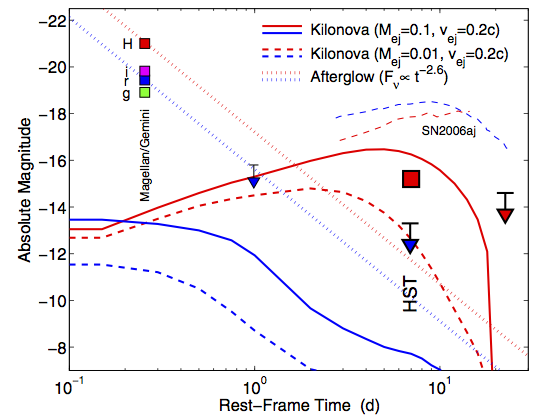
\includegraphics[scale=0.85]{figs/transients/kilonovaBerger.png}
\caption{Kilonova signature in the short GRB\,130603B as revealed by the
Hubble Space Telescope (HST). The Magellan and Gemini telescopes sampled
the optical afterglow of the GRB (dotted lines). The kilonova light
starts to dominate the emission in the H band around a few days after
the merger. Thick and dashed lines: theoretical kilonova models from
\citet{Barnes13} showing that kilonovae are fast-evolving, faint and red
transients. The light-curve of the SN\,2006aj associated with the long
GRB\,060218  is also shown for comparison. From \citet{Berger13}.}
\label{Fig:kilonova}
\end{figure}


% --------------------------------------------------------------------

\subsection{OpSim Analysis and Discussion}
\label{sec:\secname:analysis}

Effective follow up of GW triggers relies on the capability to sample a
relatively large portion of the sky, repeatedly, over a time scale $<1$
week, with different filters \citep{Cowperthwaite15}. In the optical
band, the kilonova signature is expected to be more prominent in the
$i$, $z$  and $y$ filters, which we identify as the most promising
filters for the kilonova search. We emphasize however that another set
of contemporaneous observations in  a ``bluer" filter is necessary to
acquire color information and distinguish kilonovae from other
fast-evolving transients.

We use the median inter-night gap  for visits in the same filter derived
from the candidate Baseline Cadence \texttt{minion\_1016} to show that,
in the absence of a Target of Opportunity (ToO) capability, it is
\emph{not} possible for LSST  to play a major role in the identification
of EM counterparts of GW triggers.

To identify kilonova candidates we need at least 2 observations acquired
within $\sim 1$ week  of the GW event \citep{Cowperthwaite15}. Using the
inter-night gap distribution for visits in the $y$ filter (which is the
most promising filter for a kilonova search), the area of the sky
covered with cadence  $\Delta t<7$ days at any given time, is
$A_{sky}\sim 3000$ deg$^2$ (including deep drilling fields).  This is
the area that can be searched for fast evolving transients.  Two
important considerations follow:

\begin{itemize}
\item[(1)] $A_{sky}$ only covers $P\sim7$\% of the sky. The  probability
that the \emph{entire} GW localization region is contained, by chance,
within $A_{sky}$ is thus very small.
\item[(2)] Even if LSST is able to cover a meaningful portion of the GW
region, we would still not have color information, and we would thus be
unable to filter out contaminating transients.
\end{itemize}

\textbf{We conclude that relying on the serendipitous alignment of the
LSST fields with the GW localization map is not an effective strategy to
follow up GW triggers and identify their EM counterparts. We thus
strongly recommend a ToO capability as part of the baseline LSST
operations strategy.}

Ideally, the ToO capability will allow for imaging of the GW
localization map at least twice over $\Delta t\lesssim$1 week with a
``red" filter ($i$, $z$  or $y$),  and  will include the possibility to
designate a desired set of filters to obtain color information. By the
time of LSST operation the typical size of the GW localization region is
expected to be 10-100 deg$^2$, which would require a small number of
LSST re-pointings. We thus do \emph{not} anticipate a significantly
disruptive impact on other LSST campaigns (especially if only the GW
triggers with the best localizations in the southern sky are selected
for LSST ToOs).

\textbf{At the price of re-shuffling a reasonably small number of
fields, \emph{if} equipped with ToO capabilities, LSST can be the
premier player in the era of EM follow up to GW sources.}

% ====================================================================
%
% \subsection{Conclusions}
%
% Here we answer the ten questions posed in
% \autoref{sec:intro:evaluation:caseConclusions}:
%
% \begin{description}
%
% \item[Q1:] {\it Does the science case place any constraints on the
% tradeoff between the sky coverage and coadded depth? For example, should
% the sky coverage be maximized (to $\sim$30,000 deg$^2$, as e.g., in
% Pan-STARRS) or the number of detected galaxies (the current baseline but
% with 18,000 deg$^2$)?}
%
% \item[A1:] ...
%
% \item[Q2:] {\it Does the science case place any constraints on the
% tradeoff between uniformity of sampling and frequency of  sampling? For
% example, a rolling cadence can provide enhanced sample rates over a part
% of the survey or the entire survey for a designated time at the cost of
% reduced sample rate the rest of the time (while maintaining the nominal
% total visit counts).}
%
% \item[A2:] ...
%
% \item[Q3:] {\it Does the science case place any constraints on the
% tradeoff between the single-visit depth and the number of visits
% (especially in the $u$-band where longer exposures would minimize the
% impact of the readout noise)?}
%
% \item[A3:] ...
%
% \item[Q4:] {\it Does the science case place any constraints on the
% Galactic plane coverage (spatial coverage, temporal sampling, visits per
% band)?}
%
% \item[A4:] ...
%
% \item[Q5:] {\it Does the science case place any constraints on the
% fraction of observing time allocated to each band?}
%
% \item[A5:] ...
%
% \item[Q6:] {\it Does the science case place any constraints on the
% cadence for deep drilling fields?}
%
% \item[A6:] ...
%
% \item[Q7:] {\it Assuming two visits per night, would the science case
% benefit if they are obtained in the same band or not?}
%
% \item[A7:] ...
%
% \item[Q8:] {\it Will the case science benefit from a special cadence
% prescription during commissioning or early in the survey, such as:
% acquiring a full 10-year count of visits for a small area (either in all
% the bands or in a  selected set); a greatly enhanced cadence for a small
% area?}
%
% \item[A8:] ...
%
% \item[Q9:] {\it Does the science case place any constraints on the
% sampling of observing conditions (e.g., seeing, dark sky, airmass),
% possibly as a function of band, etc.?}
%
% \item[A9:] ...
%
% \item[Q10:] {\it Does the case have science drivers that would require
% real-time exposure time optimization to obtain nearly constant
% single-visit limiting depth?}
%
% \item[A10:] ...
%
% \end{description}

% ====================================================================

\navigationbar

